\chapter{Literature Review}
\label{chap:lit_review}


\section{EHDA}
\label{sec:ehda_resume}

The electrospraying of liquids herein is referred to as electrohydrodynamic atomization (EHDA). The atomization by primarily electrical (electro) forces of a liquid (hydro) that is moving (dynamic) during the atomization captures the essence of the phenomena.\cite{Grace}
That motion applies to the liquid certain velocity that is not enough to create the spray alone. Therefore, the electric field itself is the responsible for the spraying dynamics.\cite{prunet}

The stable balance between the capillary and field forces on the liquid suggest a \emph{quasi static} dynamics.
For this reason with a controlled enviroment we can reach a certain stable spraying mode as can be seen in the Figure \ref{fig:ehda_setup_ex2}.

\begin{figure}[H]
  \centering
  \resizebox{80mm}{!}{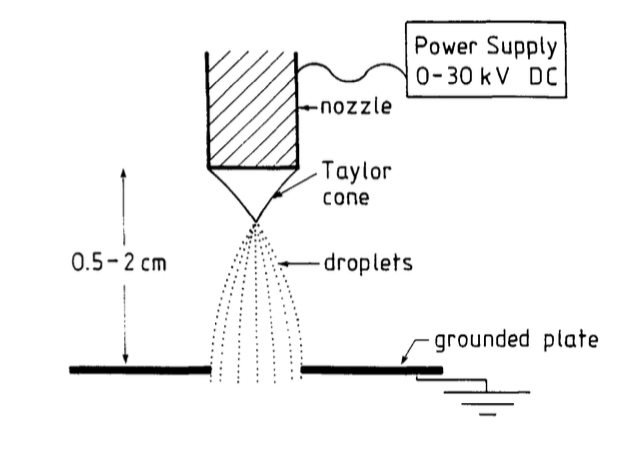
\includegraphics{Figuras/ehda_ex_2.png}}
  \caption{EHDA physical concept \cite{Gabriel}}
  \label{fig:ehda_setup_ex2}
\end{figure}


\section{Non-visual classification}
\label{sec:non-visual-classification}

From the inception of EHDA until the present day, research has been carried out through manual means, involving the use of visual classification to determine the spraying mode either through cameras or by direct observation. It is advisable to employ a high-speed camera (HS) to accurately capture the spraying process as certain intermittent or dripping states may occur at a high frequency and be erroneously perceived as a stable condition.
The setup in figure \ref{fig:ehda_setup} shows the most common setup used for EHDA researchers.

\begin{figure}[H]
  \centering
  \resizebox{90mm}{!}{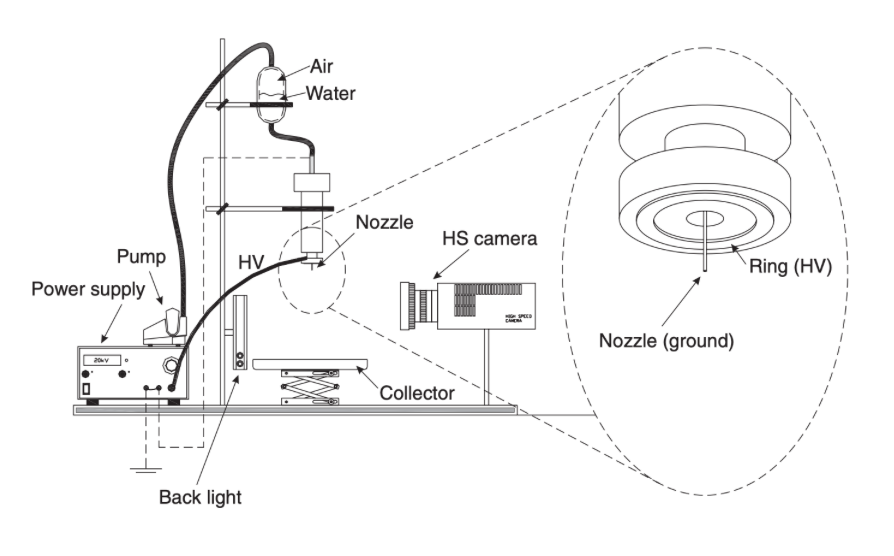
\includegraphics{Figuras/system_setup.png}}
  \caption{EHDA experiment setup \cite{Luewton}}
  \label{fig:ehda_setup}
\end{figure}


Therefore some researchs were made about the classification of the spraying mode measuring the current flowing through the nozzle to plate\cite{Sjaaks}\cite{Chen_Pui}. That current signal holds a lot o information 
about the dynamics that is happening with the liquid. Figure \ref{fig:microdripping_current_pic} illustrate an example of that. It can be seen the signal of two droplets of charged liquid generated in this time frame.


\begin{figure}[H]
    \centering
    \resizebox{150mm}{!}{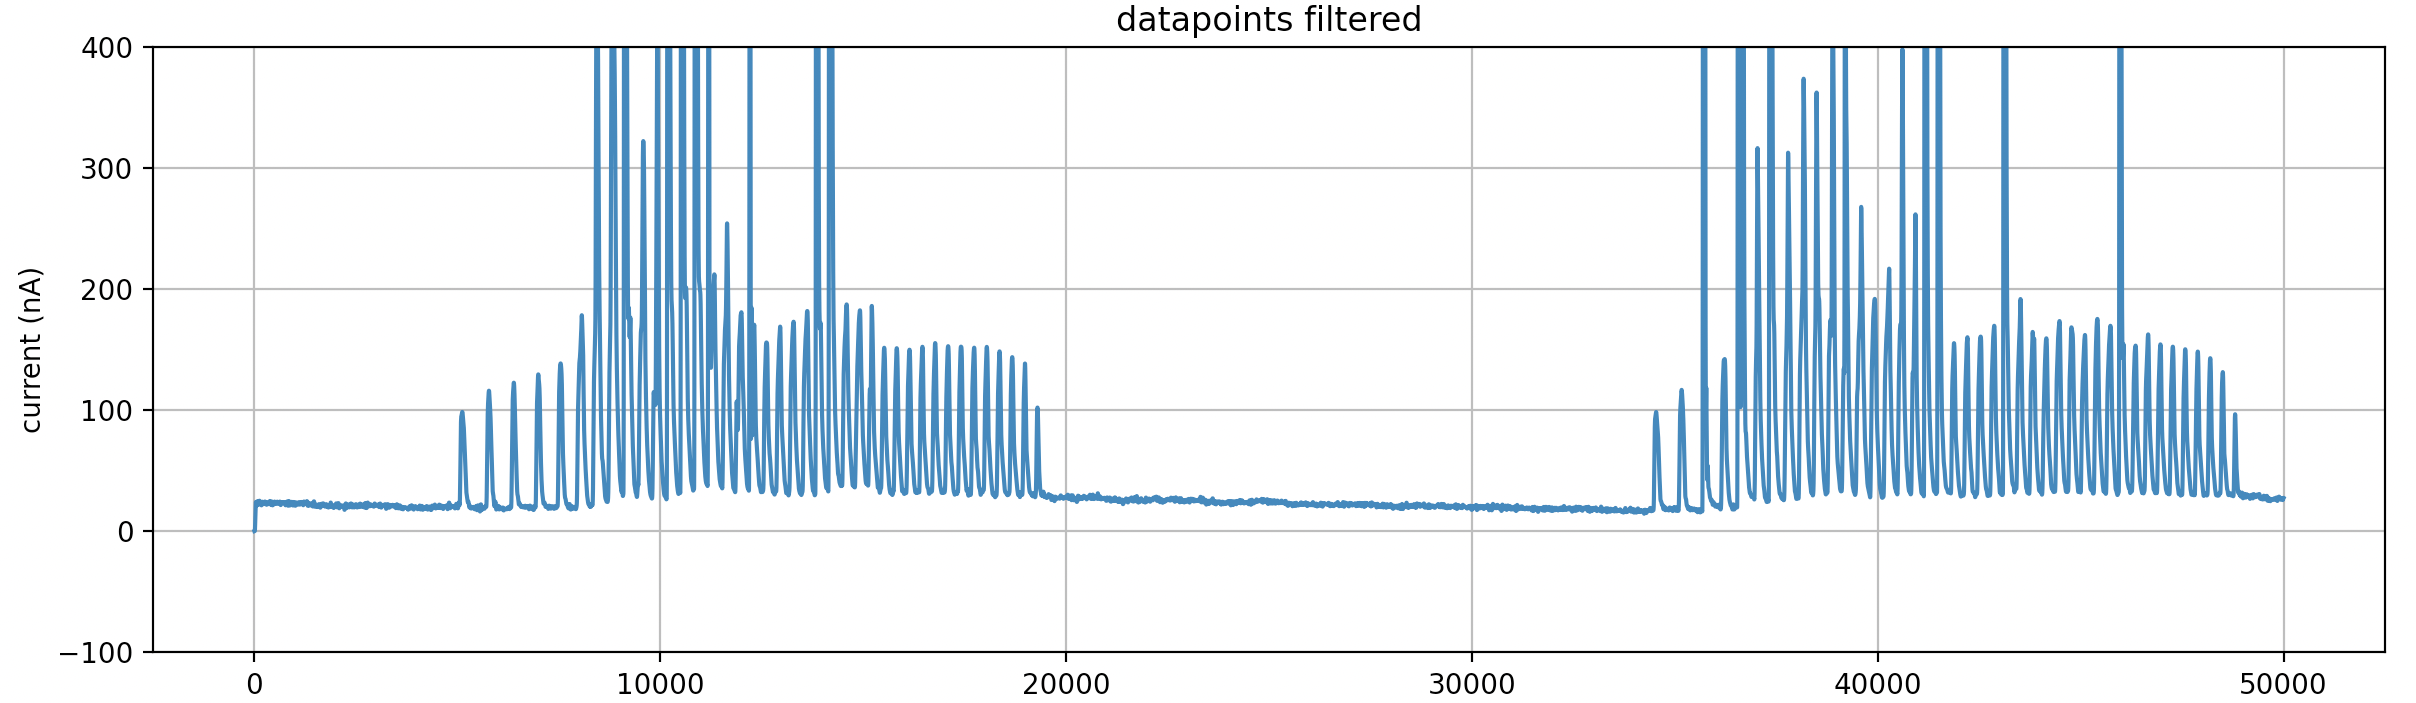
\includegraphics{Figuras/report2/img2.png}}
    \caption{Current measurement sample of a micro-dripping spraying mode. This graph represents 0.5s sample. The sampling frequency is 100kHz. Hence we have 50000 current values.}
    \label{fig:microdripping_current_pic}
  \end{figure}

  The existing signal contains valuable data not only about dripping but also other modes of spraying, thus it can serve as a non-visual classifier.
  This report draws significant inspiration from Sjaak's\cite{Sjaaks} work, which identifies distinct statistical characteristics of electrical current for various spraying modes.



\section{Scaling Laws}
\label{sec:scalling-laws}

The electric spray current is a critical variable that has been extensively researched by multiple authors\cite{prunet}\cite{Chen_Pui}\cite{gananCalvo}, resulting in scaling laws that express the relationship between liquid flow rate, conductivity, surface tension, density, and droplet diameter. 
These scaling laws can predict the size and charge of emitted droplets, making them useful tools for electrospraying practitioners. 
Obtaining scaling laws is necessary for characterizing an electrospraying system and gaining a better understanding of the process mechanisms. 

\[ I = (\frac{\gamma K Q}{\kappa})^{1/2}\]

\section{Spraying modes}
\label{sec:spraying_modes_subsec}

Since 1915 with his pioneering work in EHDA, Zeleny\cite{zeleny14} observed several functioning modes with very different characteristics.
Years later the same phenomena was noticed by other scientists, but the classification of these modes were still not well-defined by the community.
For that Cloupeau and Prunet-Foch\cite{prunet} proposed spray mode classifications based in what they have seen experimentally, and it's still being used as basis for EHDA researches.

The Figures \ref{fig:dripping_camera_example}, \ref{fig:cone_camera_jet_example}, \ref{fig:multi_camera_jet_example} shows 3 spraying dynamics that we are most interesting in this project. 

\begin{multicols}{3}

  \begin{figure}[H]
      \center
      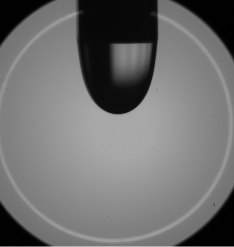
\includegraphics[width=3cm]{Figuras/drippingexample.png}
      \label{fig:dripping_camera_example}
      \caption{Dripping}
  \end{figure}


  \begin{figure}[H]
      \center
      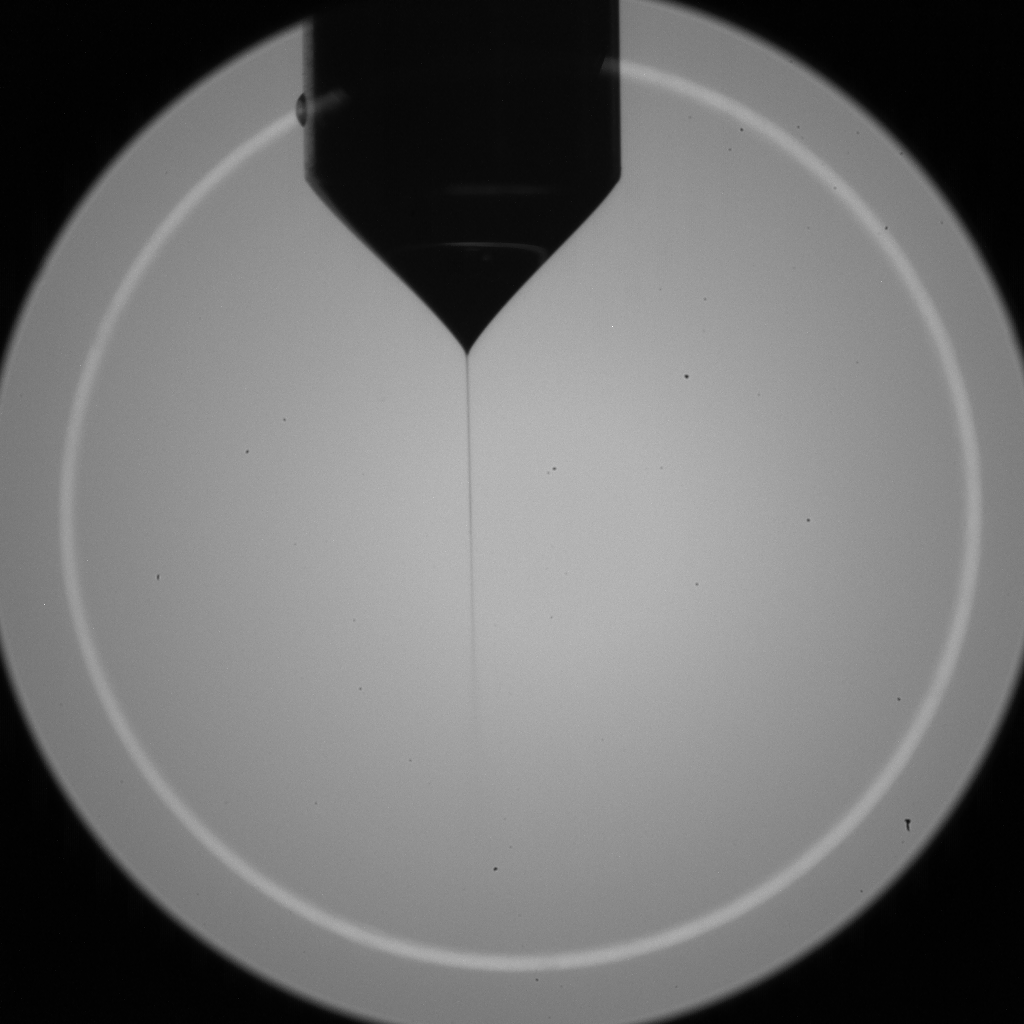
\includegraphics[width=3cm]{Figuras/conejetexample.png}
      \label{fig:cone_camera_jet_example}
      \caption{Cone Jet}
  \end{figure}


  \begin{figure}[H]
      \center
      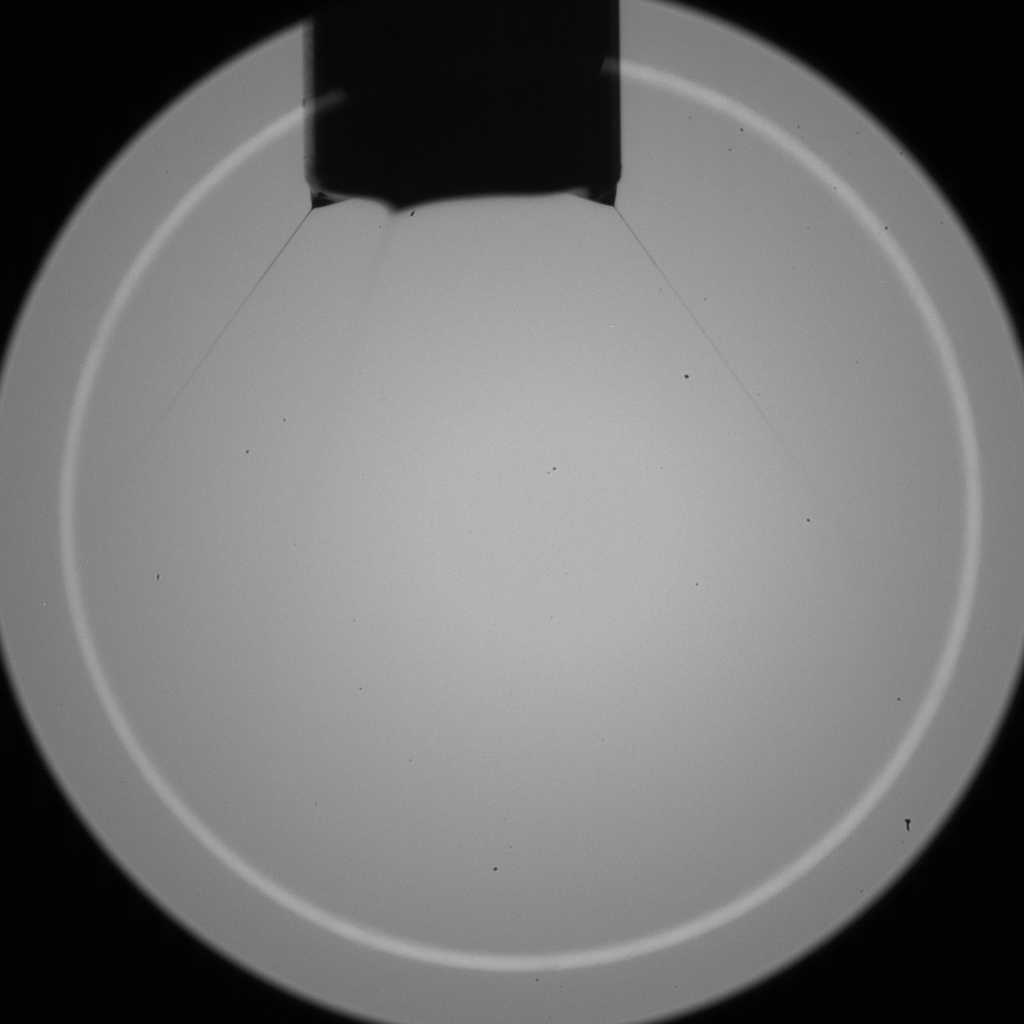
\includegraphics[width=3cm]{Figuras/multijetexample.png}
      \label{fig:multi_camera_jet_example}
      \caption{Multi Jet}
  \end{figure}

\end{multicols}


Through the various classifications and subclassifications of spraying defined in literature we are going to aggregate some of them and separate between 5 modes as shown above in order of growing electric potential:

\subsection{Dripping}
\label{subsec:dripping}

Dripping mode happens when the electric field applied is not enough to change the meniscus shape, phenomena called field enhanced dripping.
In that situation the liquid droplet has, in general, size bigger than the capillary and low frequency intervals between each drop.

\begin{figure}[H]
  \center
  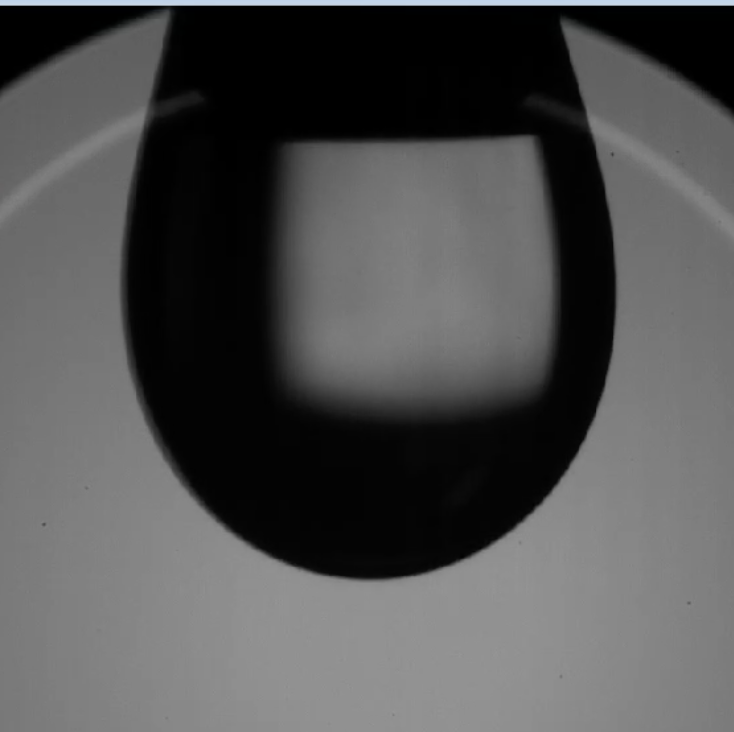
\includegraphics[width=3cm]{Figuras/19:03/drip_example.png}
  \label{fig:drip_example}
  \caption{Dripping}
\end{figure}

\subsection{Intermittent}
\label{subsec:Intermittent}

Intermittent mode is defined when the electric field forces starts to have a considerable effect in the meniscus and droplet formation. 
In this mode the droplet size is smaller than the nozzle, phenomena called microdripping, and the dripping frequency increases with the increasing of the field applied.

\begin{multicols}{3}

  \begin{figure}[H]
      \center
      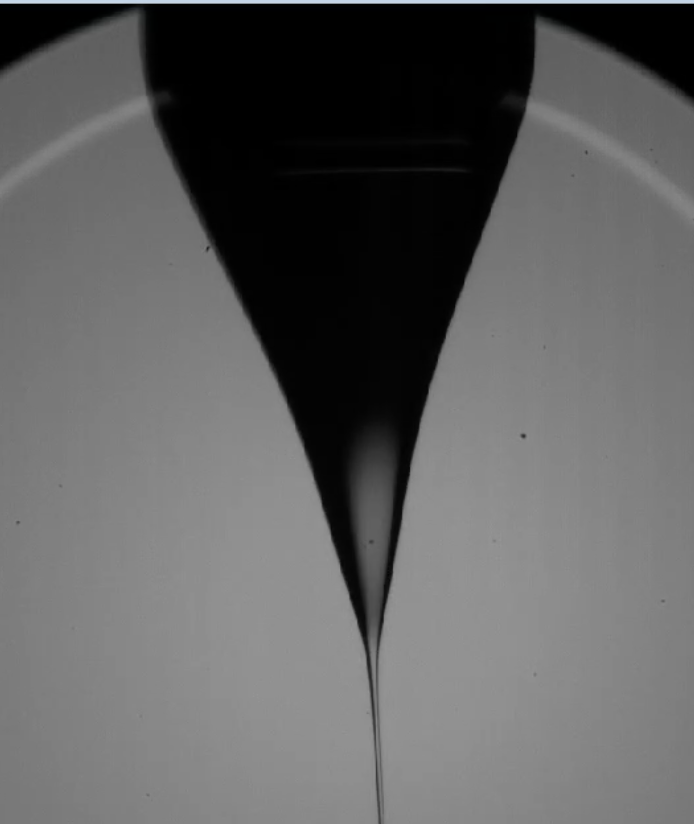
\includegraphics[width=3cm]{Figuras/19:03/intermittent_example.png}
      \label{fig:intermittent_example}
      \caption{Intermittent}
  \end{figure}


  \begin{figure}[H]
      \center
      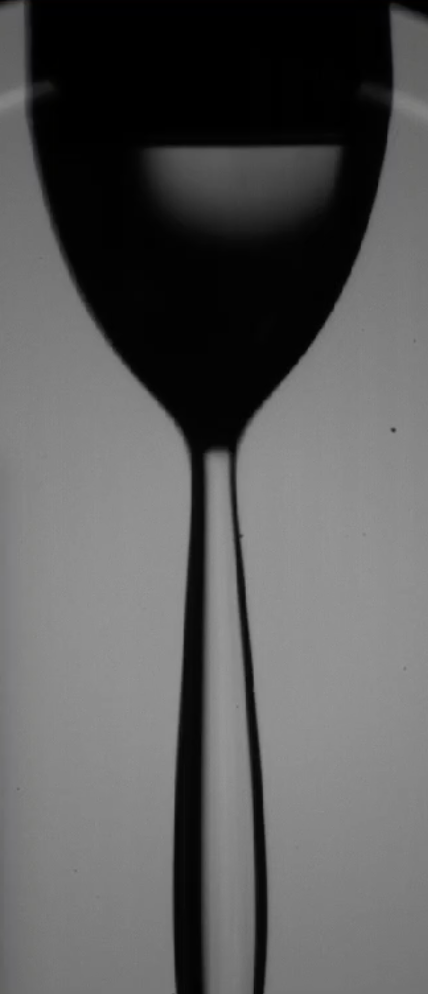
\includegraphics[width=2cm]{Figuras/19:03/intermittent2_example.png}
      \label{fig:intermittent2_example}
      \caption{Intermittent}
  \end{figure}


  \begin{figure}[H]
      \center
      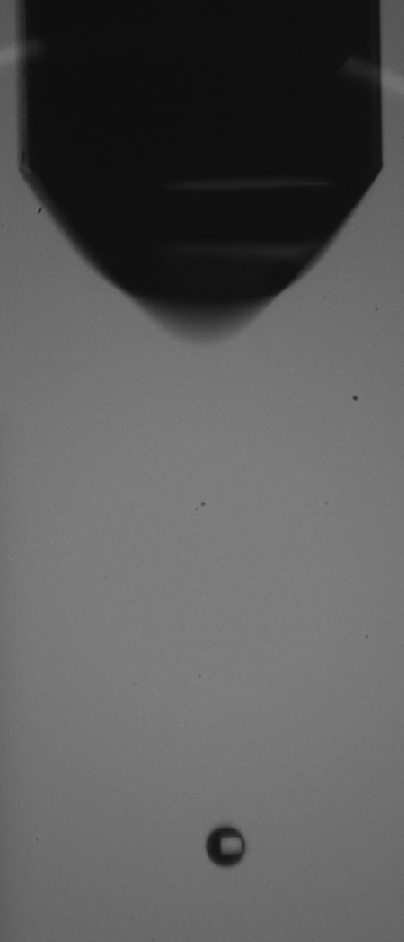
\includegraphics[width=2cm]{Figuras/19:03/microdripping_example.png}
      \label{fig:microdripping_example}
      \caption{Microdripping}
  \end{figure}

\end{multicols}

\subsection{Cone Jet}
\label{subsec:Cone Jet}

The electrified meniscus can take on a conical shape within a certain range of applied voltage and injected liquid flow rate. 


Taylor (1964)\cite{taylor} was the first to demonstrate that electrostatic pressure and capillary pressure can be balanced at any point on the surface of a liquid cone.
Taylor cone-jets naturally occurs under relatively limited circumstances: when the applied field and flow rate are in the appropriate range, and the electrosprayed liquid exhibits the adequate physical properties.

During the cone-jet, multiple parameters and variables influence the current, flow rate and voltage operational window.

\begin{multicols}{3}

  \begin{figure}[H]
      \center
      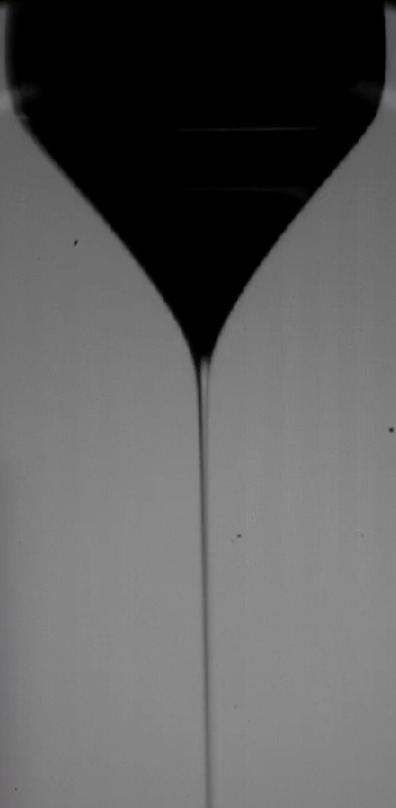
\includegraphics[width=2cm]{Figuras/april/conjet1.png}
      \label{fig:conjt1}
      \caption{Cone Jet}
  \end{figure}


  \begin{figure}[H]
      \center
      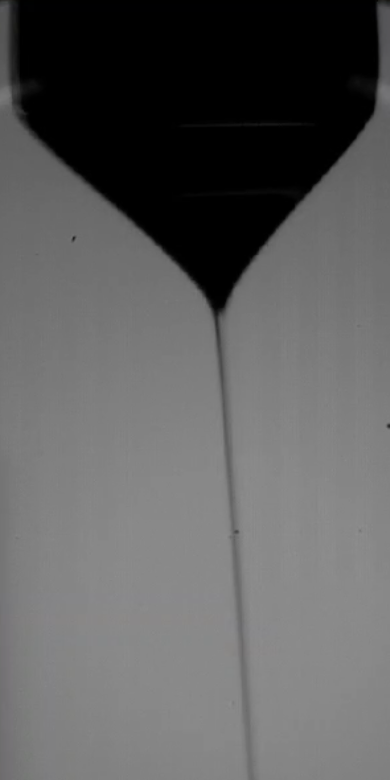
\includegraphics[width=2cm]{Figuras/april/conjet2.png}
      \label{fig:conjt2}
      \caption{Cone Jet}
  \end{figure}


  \begin{figure}[H]
      \center
      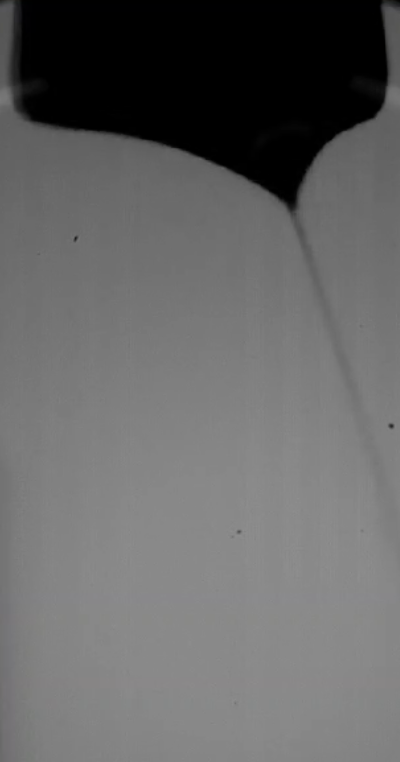
\includegraphics[width=2cm]{Figuras/april/conjet3.png}
      \label{fig:conjt3}
      \caption{Cone Jet}
  \end{figure}

\end{multicols}

\subsection{Multi Jet}
\label{subsec:Multi Jet}

Zeleny's (1915)\cite{zeleny} paper was the first reference to multi-jet phenomena. In his experiments was observed:
\emph{"for voltages well above that for which the steady conical surface changed into a blurred agitated one, the appearance became a number of fine points with their attendant dark streaks arranged along the circumference of the raised edge".}

In recent times, researchers have made significant advancements in understanding multi-jet technology and have identified various profiles with distinct characteristics. Because of that, some authors can divide what we call multi jet in more classifications.
The multi jet mode is considered in this work when two or more spraying jets can be visualized in the HS camera and the current shows a stable profile. Figures \ref{fig:multijt1}, \ref{fig:multijt2} and \ref{fig:multijt3} shows three different variations of multi jet spraying mode.

C.N. Ryan (2012)\cite{Ryan} focused his work in multi jet spraying mode, and its current properties. 
For this work it highlights the detection that for a low number of jets emitted, seen in figure \ref{fig:multijt1} and \ref{fig:multijt2}, the meniscus is not bound to the rim of the capillary. 
This mode is seen to be less stable, in that each jet in multi-jet mode is unable to support the same volumetric flow as in the single jet mode.

As the number of jets increases the mode becomes what Ryan refers at rim-mode electrospray, seen in figure \ref{fig:multijt3}. In this work it will also be classified as multi jet.



\begin{multicols}{3}

  \begin{figure}[H]
      \center
      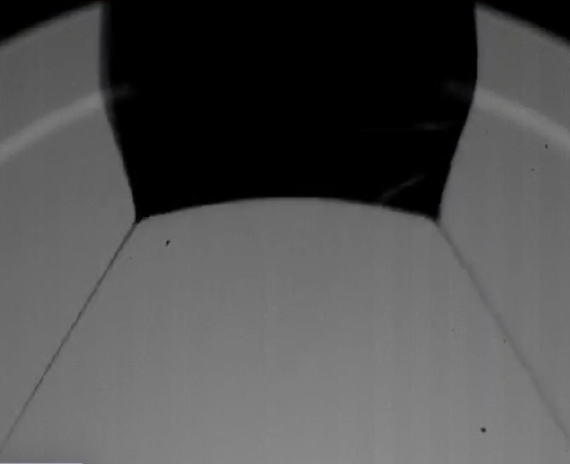
\includegraphics[width=3cm]{Figuras/april/multi2.png}
      \label{fig:multijt1}
      \caption{Multi Jet - double jet}
  \end{figure}


  \begin{figure}[H]
      \center
      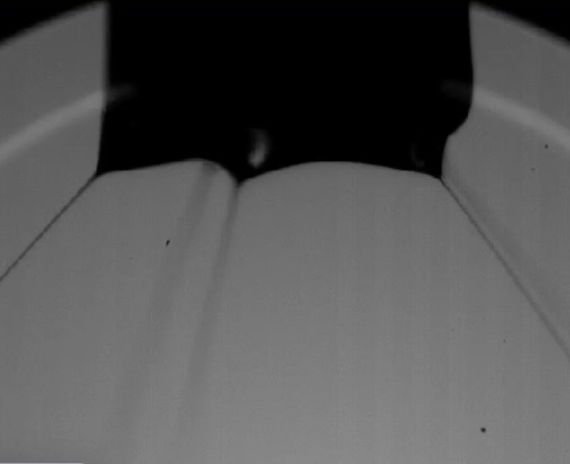
\includegraphics[width=3cm]{Figuras/april/multi1.png}
      \label{fig:multijt2}
      \caption{Multi Jet - low number of jets}
  \end{figure}


  \begin{figure}[H]
      \center
      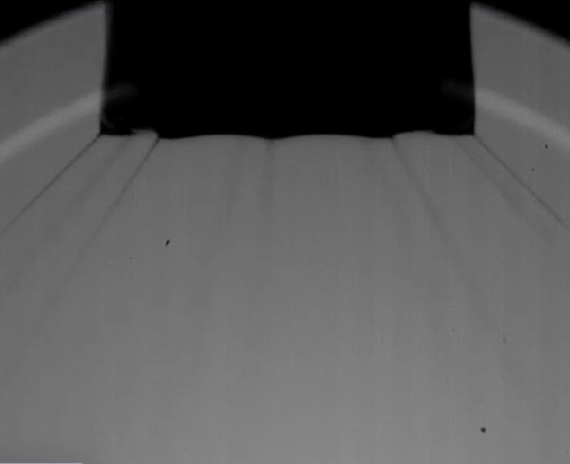
\includegraphics[width=3cm]{Figuras/april/multi3.png}
      \label{fig:multijt3}
      \caption{Multi Jet - rim spraying mode}
  \end{figure}

\end{multicols}


\subsection{Corona}
\label{subsec:Corona}

At even higher electric potentials, above of multi jet, the insulation between the electrodes start to breakdown and we achieve a phenomenon of discharge.
Those can be easily classified because of its high current value. 

This mode is also divided by other classes such as streamer corona or transient sparks discharges, but it's not in the scope of this work. 
Mônicas\cite{Monica} work was focused on how to predict that mode with the current analysis for safety in industrial applications.



\clearpage